\subsection{Rooms}
\label{subsec:application:building_the_model:rooms}

In the fourth step, the room objects will be introduced as part of the introduction of the rooms containment relation. This step introduces the $\type{rooms}$ relation on the $.\type{House}$ class, including its values. \cref{subsec:library_of_transformations:type_level_transformations:contained_class_set_fields} is used to introduce the field, while on the instance level, \cref{subsec:library_of_transformations:instance_level_transformations:contained_class_set_field_values} is used to introduce the values.

The $classtype$ of the new field is $.\type{House}$, as the field will be defined for houses. The $name$ of the new field is $\type{rooms}$ and the $containedtype$ is $.\type{Room}$. The set of objects of which the value is set is equal to all house objects, so $objects = \{TR, BHP\}$. The function for $obids$ returns the existing identifier of each of these objects. The multiplicity is set to $0..9$ for the new field, and the $values$ function is defined as follows:
\begin{equation*}
    values = \big\{\big(TR, \{TRRoom1, TRRoom2\}\big), \big(BHP, \{BHPRoomA, BHPRoomB, BHPRoomC\}\big)\big\}
\end{equation*}

Please note that the referenced objects are all new. For these new objects $obids$ returns as identifier the internal node label, just as was done for the houses. The following model is obtained:

\LTXtable{\textwidth}{tex/06_application/02_building_the_model/tables/04_rooms.tex}

\begin{figure}[p]
    \centering
    \begin{subfigure}{0.98\textwidth}
        \centering
        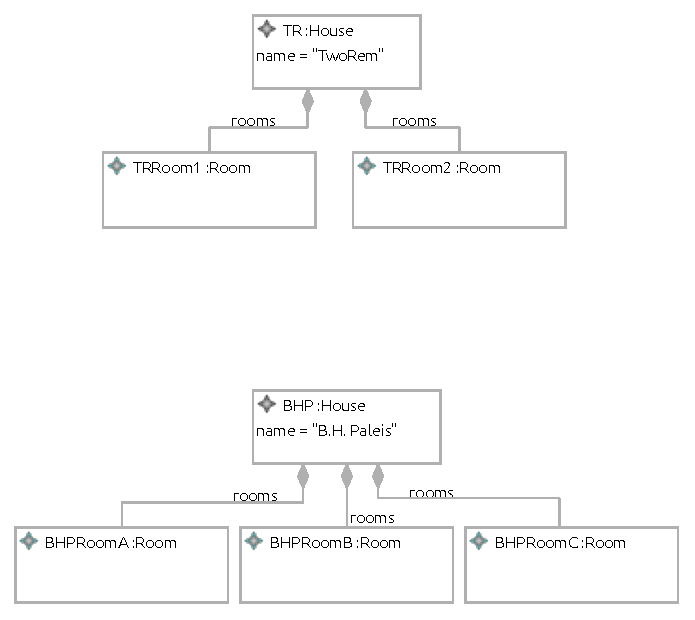
\includegraphics{images/06_application/instance_model/step04.pdf}
        \caption{Instance Model $Im_4$}
        \label{fig:application:building_the_model:rooms:ecore:instance_model}
    \end{subfigure}
    \\
    \begin{subfigure}{0.98\textwidth}
        \centering
        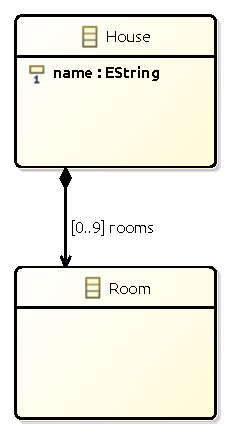
\includegraphics{images/06_application/type_model/step04.pdf}
        \caption{Type Model $Tm_4$}
        \label{fig:application:building_the_model:rooms:ecore:type_model}
    \end{subfigure}
    \caption{The Ecore model after step 4}
    \label{fig:application:building_the_model:rooms:ecore}
\end{figure}

\begin{figure}[p]
    \centering
    \begin{subfigure}{0.98\textwidth}
        \centering
        % To use this figure in your LaTeX document
% import the package groove/resources/groove2tikz.sty
%
\begin{tikzpicture}[scale=\tikzscale,name prefix=step04-]
\node[basic_node] (n0) at (2.740, -4.200) {\ml{\uline{\textit{BHP}} : \textbf{House}\\name = "B.H. Paleis"}};
\node[basic_node] (n1) at (2.660, -0.340) {\ml{\uline{\textit{TR}} : \textbf{House}\\name = "TwoRem"}};
\node[basic_node] (n7) at (1.820, -1.470) {\ml{\uline{\textit{TRRoom1}} : \textbf{Room}}};
\node[basic_node] (n8) at (3.410, -1.480) {\ml{\uline{\textit{TRRoom2}} : \textbf{Room}}};
\node[basic_node] (n14) at (0.820, -3.060) {\ml{\uline{\textit{BHPRoomA}} : \textbf{Room}}};
\node[basic_node] (n15) at (2.780, -3.050) {\ml{\uline{\textit{BHPRoomB}} : \textbf{Room}}};
\node[basic_node] (n16) at (4.720, -3.060) {\ml{\uline{\textit{BHPRoomC}} : \textbf{Room}}};

\path[basic_edge] (n0)  --  (n14) 
node[lab] at (1.584, -3.455) {\ml{rooms}};
\path[basic_edge](n0.north -| 2.780, -3.050) -- node[lab] {\ml{rooms}} (n15) ;
\path[basic_edge] (n0)  -- node[lab] {\ml{rooms}} (n16) ;
\path[basic_edge] (n1)  -- node[lab] {\ml{rooms}} (n7) ;
\path[basic_edge] (n1)  -- node[lab] {\ml{rooms}} (n8) ;
\end{tikzpicture}

        \caption{Instance Graph $IG_4$}
        \label{fig:application:building_the_model:rooms:groove:instance_graph}
    \end{subfigure}
    \\
    \begin{subfigure}{0.98\textwidth}
        \centering
        % To use this figure in your LaTeX document
% import the package groove/resources/groove2tikz.sty
%
\begin{tikzpicture}[scale=\tikzscale,name prefix=step04-]
\node[basic_node] (n0) at (2.740, -4.200) {\ml{\uline{\textit{BHP}} : \textbf{House}\\name = "B.H. Paleis"}};
\node[basic_node] (n1) at (2.660, -0.340) {\ml{\uline{\textit{TR}} : \textbf{House}\\name = "TwoRem"}};
\node[basic_node] (n7) at (1.820, -1.470) {\ml{\uline{\textit{TRRoom1}} : \textbf{Room}}};
\node[basic_node] (n8) at (3.410, -1.480) {\ml{\uline{\textit{TRRoom2}} : \textbf{Room}}};
\node[basic_node] (n14) at (0.820, -3.060) {\ml{\uline{\textit{BHPRoomA}} : \textbf{Room}}};
\node[basic_node] (n15) at (2.780, -3.050) {\ml{\uline{\textit{BHPRoomB}} : \textbf{Room}}};
\node[basic_node] (n16) at (4.720, -3.060) {\ml{\uline{\textit{BHPRoomC}} : \textbf{Room}}};

\path[basic_edge] (n0)  --  (n14) 
node[lab] at (1.584, -3.455) {\ml{rooms}};
\path[basic_edge](n0.north -| 2.780, -3.050) -- node[lab] {\ml{rooms}} (n15) ;
\path[basic_edge] (n0)  -- node[lab] {\ml{rooms}} (n16) ;
\path[basic_edge] (n1)  -- node[lab] {\ml{rooms}} (n7) ;
\path[basic_edge] (n1)  -- node[lab] {\ml{rooms}} (n8) ;
\end{tikzpicture}

        \caption{Type Graph $TG_4$}
        \label{fig:application:building_the_model:rooms:groove:type_graph}
    \end{subfigure}
    \caption{The GROOVE graphs after step 4}
    \label{fig:application:building_the_model:rooms:groove}
\end{figure}

A visual representation of $Tm_4$ and $Im_4$ can be found in \cref{fig:application:building_the_model:rooms:ecore}. Similarly, a visual representation of $TG_4$ and $IG_4$ can be found in \cref{fig:application:building_the_model:rooms:groove}. Please note that because of the definitions of $f_4(Im_4)$ and $f'_4(IG_4)$, we have that $f_4(Im_4) = IG_4$ and $f'_4(IG_4) = Im_4$. Furthermore, $f_4(Im_4)$ and $f'_4(IG_4)$ are valid mapping functions themselves, such that they can be combined with another mapping function in the next step.

The introduction of the room objects makes that the model represents something. A house has rooms that it contains, and each house has a different set of rooms. Still, there is room to enlarge the model more, such that more details are included.

\afterpage{\FloatBarrier}